\section{Supplementary Information}
\label{sec:conc}
\subsection{Site Intercomparison of Baring Head and Cape Grim}
\begin{figure}[h!]
  \caption{ Intercomparison of ${\Delta^{14}CO_{2}}$ measurements  at Cape Grim, Tasmania (CGO), and Baring Head, New Zealand (BHD) collected by NIWA and measured at Rafter Radiocarbon Laboratory. Dates represent the middle of the sampling period, which differ no more than one day between sites. These data show that during the time in which data are available, no measureable difference is found between the two sites. This provides some evidence that the two sites may be considered equivalent for this intercomparability study.}
% This data originally was sent to me in Jocelyn's first dropbox file. Later it was condensed to the currnent file in the H: drive.  H:\Science\Datasets\CGOvBHD
  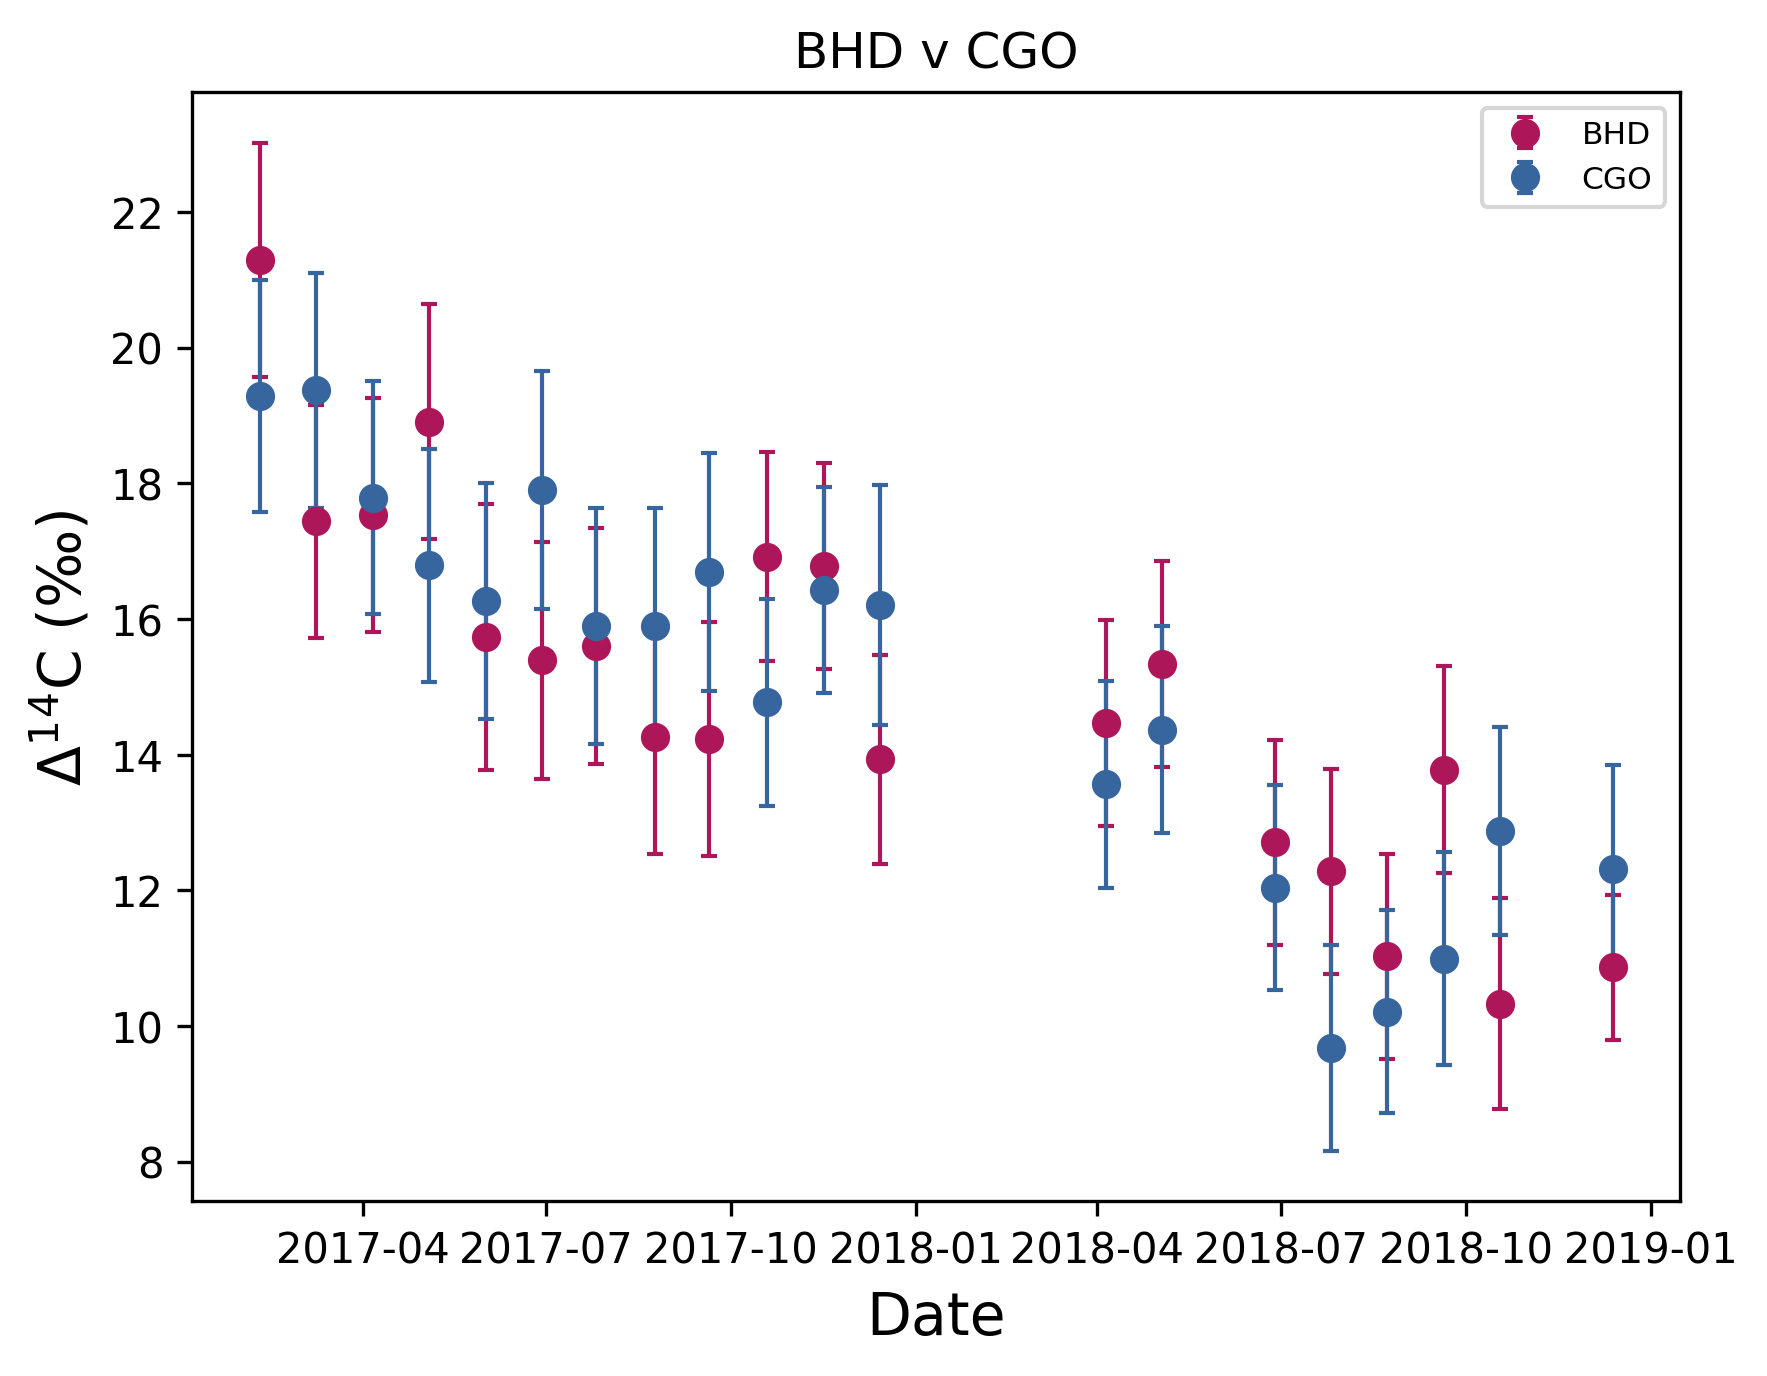
\includegraphics[width=1\textwidth]{/mnt/c/Users/clewis/IdeaProjects/GNS/Interlab_Comparison/output/Site_intercomparison.png}
\label{fig:bhdvcgo}
\end{figure}

\subsection{Removal of data interval 2009 - 2012 in Rafter vs. Heidelberg University Intercomparison}
